%--------------------
% Packages
% -------------------
\documentclass[11pt,a4paper]{article}


\usepackage[pdftex]{graphicx} % Required for including pictures
\usepackage[pdftex,linkcolor=black,pdfborder={0 0 0}]{hyperref} % Format links for pdf
\usepackage{calc} % To reset the counter in the document after title page

\frenchspacing % No double spacing between sentences
\linespread{1.2} % Set linespace
\usepackage[a4paper, lmargin=0.1666\paperwidth, rmargin=0.1666\paperwidth, tmargin=0.1111\paperheight, bmargin=0.1111\paperheight]{geometry} %margins

\usepackage[protrusion=true,expansion=true]{microtype} % Improves typography, load after fontpackage is selected


%-----------------------
% Set pdf information and add title, fill in the fields
%-----------------------
\hypersetup{
pdfsubject = {Software Product Engineering},
pdftitle = {SCEEM Space - Requirements},
pdfauthor = {Jason Park, Sungijn Kang, William Nafack, Calum West}
}

%-----------------------
% Begin document
%-----------------------
\begin{document}

\begin{titlepage}
   \vspace*{\stretch{1.0}}
   \begin{center}
      \Large\textbf{SCEEM Space - Requirements}\\
      \large\textit{Jason Park, Sungijn Kang, William Nafack, Calum West}
   \end{center}
   \vspace*{\stretch{2.0}}
\end{titlepage}

\section{Requirements}
\subsection{Client requirements}
Through meetings with our client, we were able to compile a list of their specific requirements for the system we were building. The main requirement for the system was that they wanted a dynamic website application instead of a static Excel spreadsheet. These are some of the other requirements outlined by the client.

\begin{itemize}
    \item There needs to be three different kinds of members: Professor, Lecturer, PhD Student
    \item It should be possible to sort for each different type of member.
    \item It should be possible to designate a room type for each room in every location.
    \item It should be possible to sort by room type.
    \item Staff members need to be able to find out how many people can be allocated to a specific location.
    \item There needs to be a login system.
\end{itemize}

From this list of requirements, we created a simple table comparing what our system would be able to do compared to what the previous spreadsheet was unable to accommodate.

\begin{table}[ht]
\centering
\begin{tabular}{|p{0.5\textwidth}|p{0.5\textwidth}|}
\hline
Developed Website Application & Excel Spreadsheet  \\
\hline
Multiple staff can use the website at the same time & Multiple access not possible\\
Automatic calculation of remaining spaces in a location & Remaining spaces in a location have to be counted by hand\\
Automatic detection of duplicated member ID's or emails & Manual detection of duplicated member ID's or emails\\
Easy reallocation of members' locations & Difficult reallocation of members' locations\\
Automatically sorting members by priority & Manual checking of members' priorities\\
Automatic sorting of allocations' expiry dates & Manually removing allocations once expiry dates have been reached\\
\hline
\end{tabular}
\end{table}

We were then able to identify both user and non-user stakeholders of our system and specific requirements relating to each stakeholder. This then allowed us to produce different flow steps for the system, as well as alternative and exceptional flow steps.

\subsection{Identified user stakeholders for SCEEM Space:}
\begin{itemize}
    \item \textit{Staff members} of ‘The School of Computer Science, Electrical and Electronic Engineering and Engineering Maths’. These staff members are admins that have access to the SCEEM Space application and can make changes, update information, add/remove people.
\end{itemize}

\subsection{User stakeholder stories:}
These are some different 'user stories'. They are things that the user (staff members) want to be able to do when they are using the product:
\begin{itemize}
        \item Quick and easy way to add/remove locations as the school moves/expands  into different buildings.
        \item Quick and easy way to add/remove desks as more spaces become available to the school in different locations.
        \item Quick and easy way to add/remove members as people become members of the university, or leave the university.
        \item Manage sensitive information for academics and PhD students (names, emails, ID's, groups).
        \item Need to keep track of how many members are assigned to each group, therefore allowing a count of locations assigned to each group.
        \item Be able to keep track of the total number of locations, see how many are free and how many are allocated to a member.
    \end{itemize}

\subsection{Identified stakeholders for SCEEM Space:}
\begin{itemize}
    \item \textit{Academics (Professors/Lecturers)} don’t have direct access to the database and other persons information contained within the database. They will not be able to see where other people are located office/desk wise. They are stakeholders as they are affected by the information input into the system by the staff members.
    \item \textit{PhD students} don’t have direct access to the database and other persons information contained within the database. They will not be able to see where other people are located office/desk wise. They are stakeholders as they are affected by the information input into the system by the staff members.
    \item \textit{University students} are not directly affected by the system but are still stakeholders. This system is used to assign spaces to academics and PhD students, and since university students often need to go to lecturers offices, the students are indirectly affected by where academics and PhD students are placed by the system. If an academic were to request to move office and this was accommodated by the system, then a university student would now have to go to a different place to speak to this academic.
\end{itemize}

\subsection{Flow steps for user stakeholder (staff member) stories:}
\begin{itemize}
  \item Add location:
    \begin{itemize}
      \item Navigate to application login page
      \item Login to application using provided admin login details
      \item Navigate to 'Register Location' tab
      \item Enter details of location (name, room type, no. of desks)
    \end{itemize}
  \item Remove location:
    \begin{itemize}
      \item Navigate to application login page
      \item Login to application using provided admin login details
      \item Navigate to ‘Registered Locations’ tab
      \item Find location to be removed
      \item Click on 'Delete' next to location
    \end{itemize}
  \item Add desk to location:
    \begin{itemize}
      \item Navigate to application login page
      \item Login to application using provided admin login details
      \item Navigate to ‘Registered Locations’ tab
      \item Find location in which the desk will be added
      \item Click on ‘Modify' button
      \item Change details of the location to add a desk
    \end{itemize}
  \item Remove desk from location:
    \begin{itemize}
      \item Navigate to application login page
      \item Login to application using provided admin login details
      \item Navigate to ‘Registered Locations’ tab
      \item Find location in which the desk will be removed from
      \item Click on ‘Modify’ button
      \item Change details of location to remove a desk
    \end{itemize}
\newpage
  \item Add member:
    \begin{itemize}
      \item Navigate to application login page
      \item Login to application using provided admin login details
      \item Navigate to ‘Register Member’ tab
      \item Enter details of ‘member’ e.g Name, Email, Group, Pathway etc.
    \end{itemize}
  \item Remove member:
    \begin{itemize}
      \item Navigate to application login page
      \item Login to application using provided admin login details
      \item Navigate to ‘Registered Members' tab
      \item Find member to remove
      \item Click on 'Delete' button next to member
    \end{itemize}
  \item Allocate member to location:
    \begin{itemize}
        \item Navigate to application login page
        \item Login to application using provided admin login details
        \item Navigate to 'Allocate Member' tab
        \item Select 'member' from drop-down list
        \item Select 'location' from drop-down list
        \item Enter other information (desk no., end date)
    \end{itemize}
  \item Remove member from location:
    \begin{itemize}
        \item Navigate to application login page
        \item Login to application using provided admin login details
        \item Navigate to 'Allocate Members/Locations' tab
        \item Search for 'member' using search bar
        \item Click 'Remove' button next to 'member'
    \end{itemize}
  \item Manage sensitive information:
    \begin{itemize}
      \item Navigate to application login page
      \item Login to application using provided admin login details
      \item Navigate to ‘Registered Members’ tab
      \item Search for ‘member’ using search bar
      \item Click on ‘Modify'
      \item Change any details that need to be added/removed
    \end{itemize}
  \item Access total number of free desks/offices:
    \begin{itemize}
      \item Navigate to application login page
      \item Login to application using provided admin login details
      \item Navigate to ‘Registered Locations’ tab
      \item Look at number of desks left in each location
    \end{itemize}
\end{itemize}

\subsection{Alternative flows:}
\begin{itemize}
  \item Manage sensitive information:
    \begin{itemize}
        \item Navigate to application login page
        \item Login to application using provided admin login details
        \item Navigate to 'Registered Members' tab
        \item Click on 'Delete' button for 'member' you would like to change
        \item Navigate back to home page
        \item Navigate to 'Register Member' tab
        \item Enter details of 'member' different to original details
    \end{itemize}
  \item Access total number of free desks/offices:
    \begin{itemize}
        \item Navigate to application login page
        \item Login to application using provided admin login details
        \item Navigate to 'Allocated members/locations' tab
        \item Count number of members allocated to location
        \item Subtract total number of allocated members from total number of locations
    \end{itemize}
\end{itemize}

\subsection{Exceptional flows:}
\textit{Exceptional} flow steps are shown in italics.
\begin{itemize}
  \item Add location:
    \begin{itemize}
       \item Navigate to application login page
       \item Login to application using provided admin login details
       \item \textit{Navigate to incorrect tab}
       \item Navigate to 'Register Location' tab
       \item \textit{Click on 'Submit' button}
       \item \textit{Enter incorrect details for space}
       \item Enter correct details for space
       \item Click on 'Submit' button
    \end{itemize}
\end{itemize}

\subsection{Functional and Non-Functional requirements:}
From some of the goals of the system, we have taken the flow-steps and decomposed them into both functional and non-function requirements.

\begin{itemize}
    \item Functional Requirements:
        \begin{itemize}
            \item Member:
                \begin{itemize}
                    \item Sort by member number (ascending/descending)
                    \item Sort by priority of member
                    \item Sort by department of member
                    \item Sort by pathway of member
                \end{itemize}
            \item Location:
                \begin{itemize}
                    \item Sort by location name
                    \item Sort by room type
                    \item Show unoccupied desks in a particular location
                \end{itemize}
            \item Allocated member/location:
                \begin{itemize}
                    \item Search member by member number
                    \item Search location by location name
                    \item Sort by expiry date
                    \item Sort by allocation status (allocated, unallocated)
                    \item Allocation history should be available
                \end{itemize}
            \item Account page:
                \begin{itemize}
                    \item Register account
                    \item Delete account
                \end{itemize}
        \end{itemize}
    \item Non-Functional Requirements:
        \begin{itemize}
            \item Deleting a member:
                \begin{itemize}
                    \item Instead of deleting a member, modify all details as 'None' or 'N/A'
                    \item Use deleted member when registering new member if available
                \end{itemize}
            \item Deleting a location:
                \begin{itemize}
                    \item Instead of deleting a location, modify all details as 'None' or 'N/A'
                    \item Use deleted location when registering new location if available
                \end{itemize}
            \item Re-allocation:
                \begin{itemize}
                    \item First remove, then allocate again
                \end{itemize}
        \end{itemize}
\end{itemize}

The non-functional requirements are necessary due to the relationships between the tables implemented in the system. When a member is allocated to a location, the software creates a new table that links the member table and the location table. When we remove a member from a location, the system tries to delete a row in the table which is not possible due to the parent child relationships in SQL tables. This means details are set to 'None' or NULL instead, allowing new allocations to happen.

\subsection{High-level Use-case Diagram}
This diagram depicts a high-level relationship between use cases, actors and the system.

\begin{figure}[!h]
    \centering
    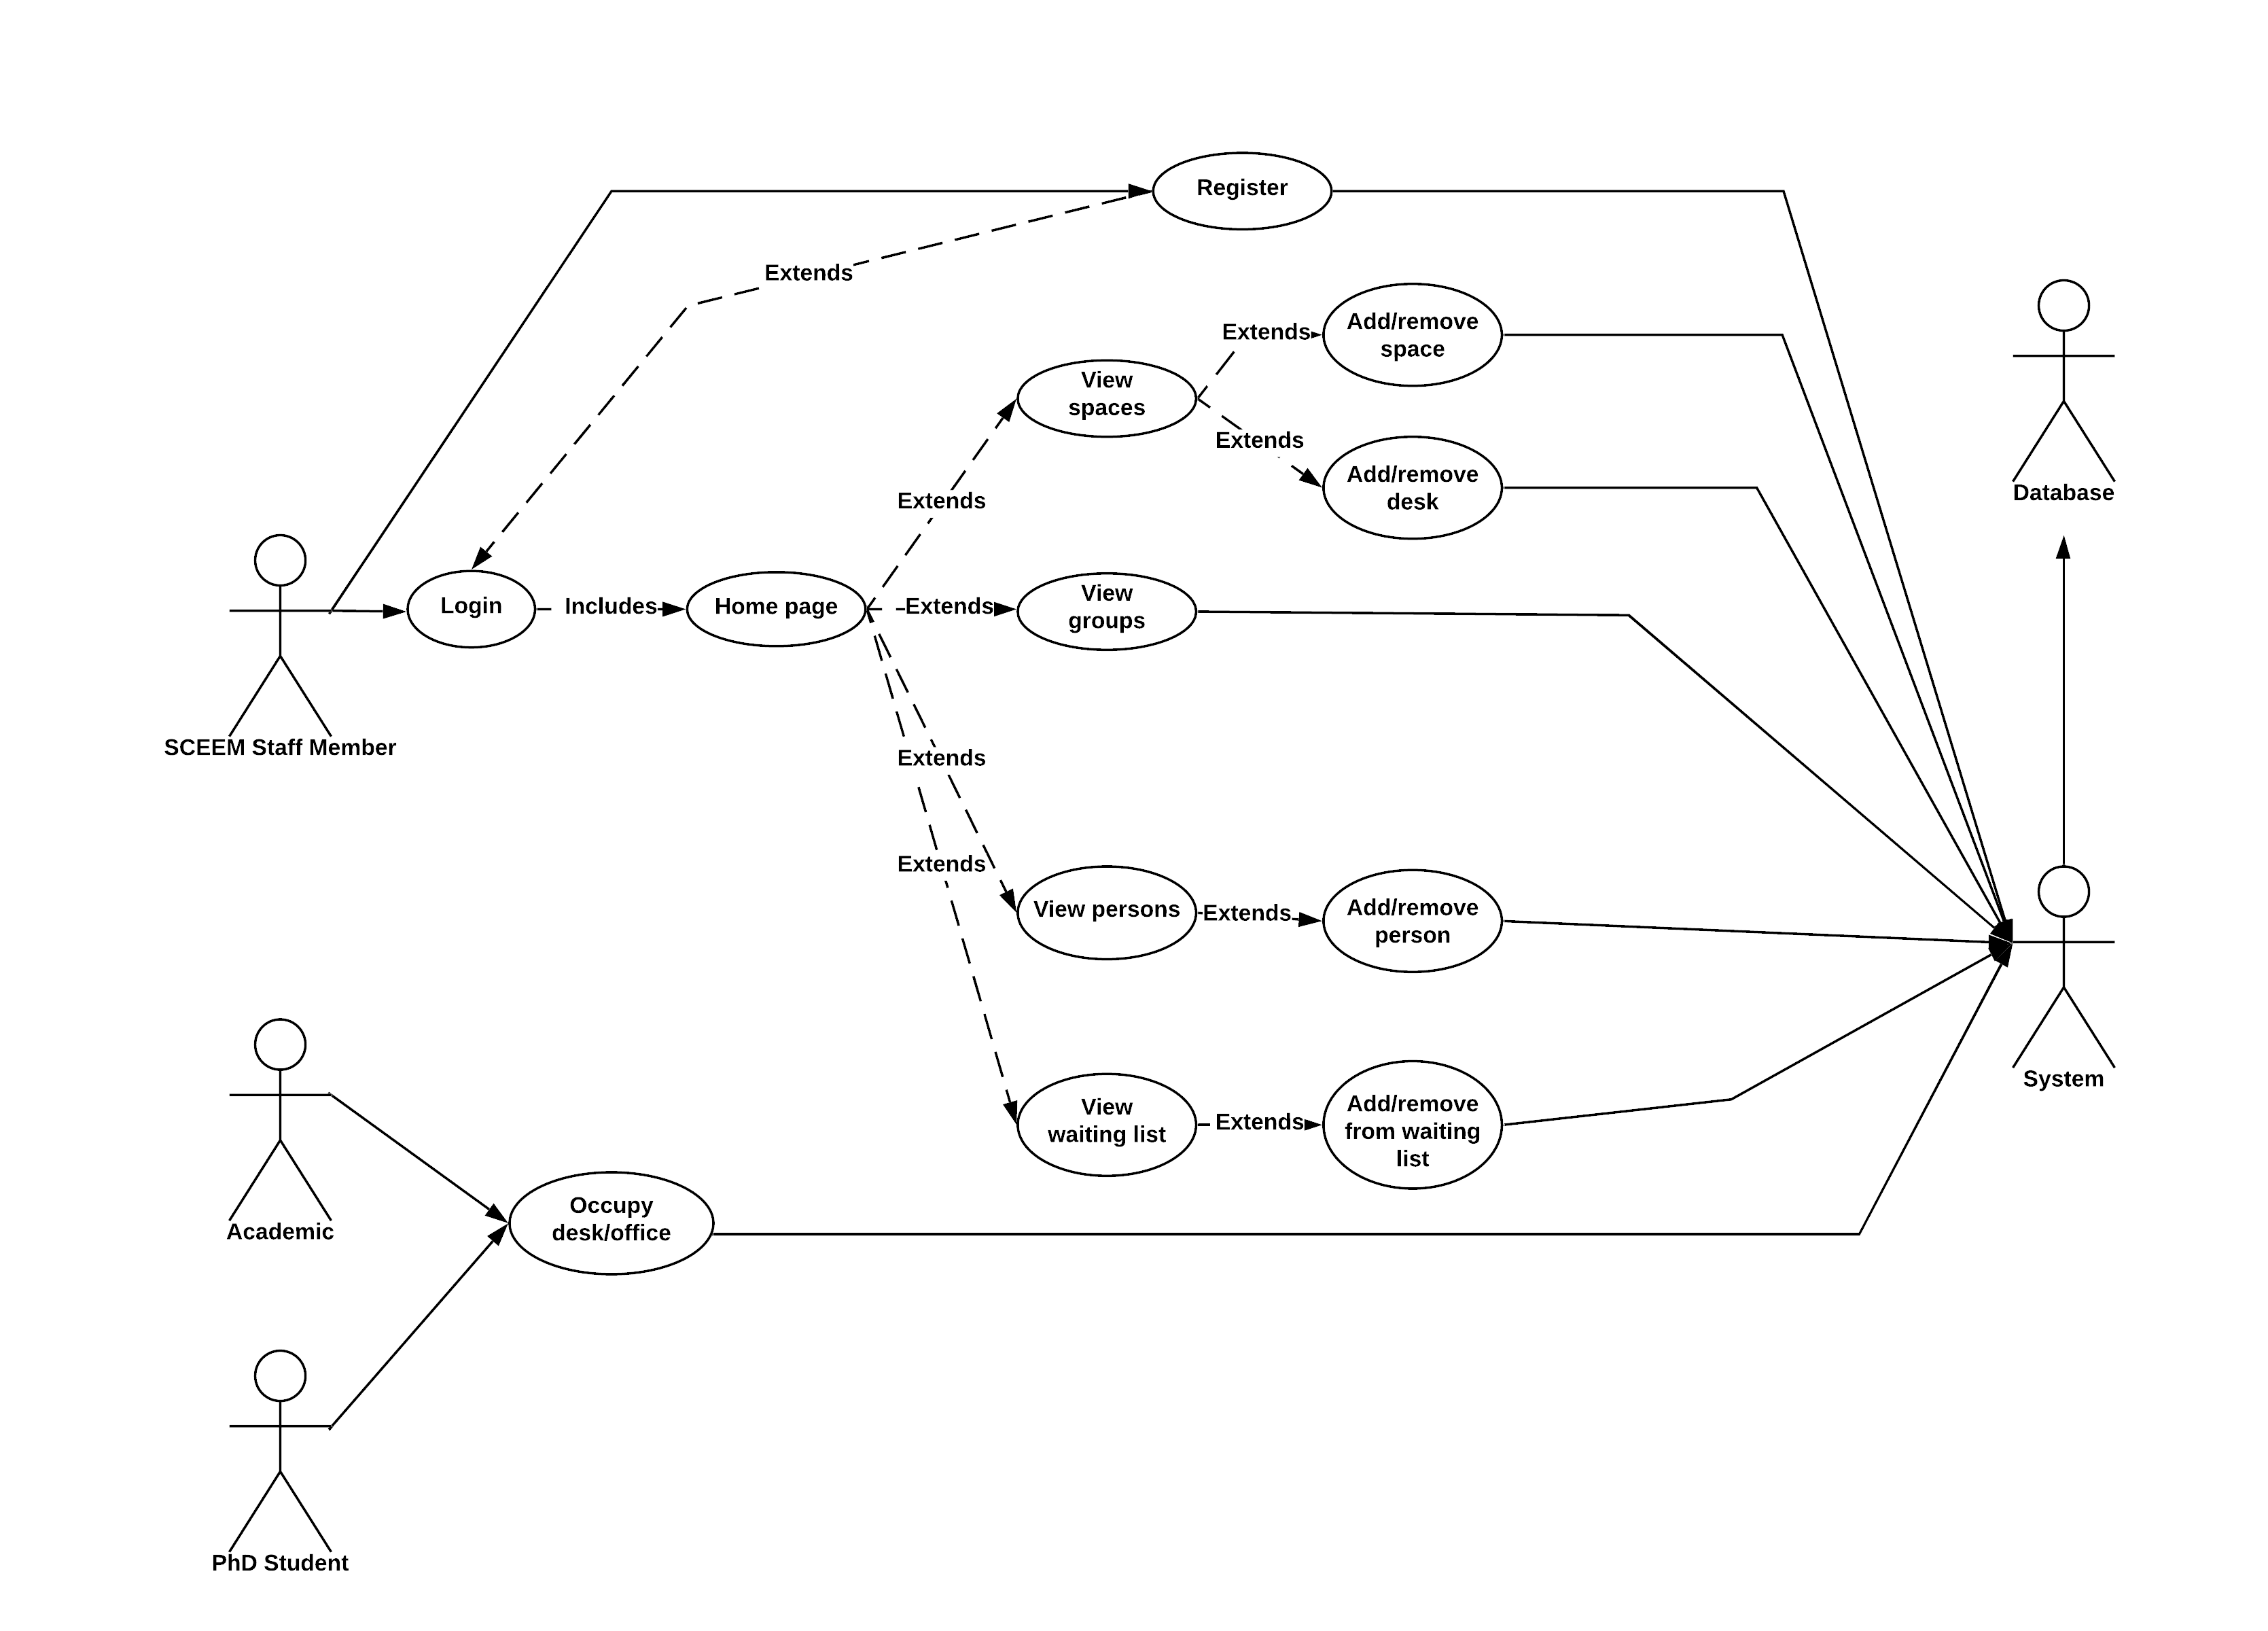
\includegraphics[width=\linewidth]{use_case.png}
    \caption{High-level Use-case diagram}
    \label{fig:basic_2}
\end{figure}

\end{document}
